% ---------------------------------------------------------------------
% ---------------------------------------------------------------------
% ---------------------------------------------------------------------

\chapter[Common strategies for the analysis of metabolomic data]{Common strategies for the analysis of metabolomic data}



% ---------------------------------------------------------------------
% ---------------------------------------------------------------------
\section{Classical bivariate tests}
\label{bivariate_tests}
As exposed in \autoref{sec:challengesmetabodata}, many metabolomic data analysis are performed using rudimentary statistical methods such as bivariate tests \parencite{saccenti2014reflections}. These tests, such as the well know \textit{t test} consist in the test of a specific hypothesis of equality for each of the variables being studied. The hypothesis test assesses for each metabolite if its mean (or median depending on the test being used) is different among the groups being compared. This way, in a study searching for biomarkers to discern between controls and patients of a specific disease, one hypothesis test (\autoref{hypotest}) for differences between both groups is performed for each of the metabolites in the data set, thus performing hundreds or thousands of hypothesis test in the analysis.

\begin{equation}
\label{hypotest}
\begin{split}
H_0: \mu_{controls} = \mu_{patients} \\
H_A: \mu_{controls} \neq \mu_{patients}
\end{split}
\end{equation}

The advantages of bivariate tests are the ease of application and interpretation of the results \parencite{vetter2018unadjusted}, but they suffer from a lot of issues. One of the most important issues when performing bivariate tests is the integration of results \parencite{katz2011multivariable}. Usually, even when finding several statistically significant biomarkers in a study, each of them has a small effect not being able by itself of discriminating between the groups being studied. Since the analysis was performed independenly on each variable, there is no way of combining the different selected biomarkers to perform a prediction, or even to understand the behavior of the studied biological system. Another important issue is the inability of controlling for confounders \parencite{heinze2017five}. Most sudies are observational, so groups are almost always never directly comparable. Bivariate tests are not able to take into account possible confounders and this renders many of their results invalid. There is also no way of assessing possible interactions among variables \parencite{hassall2018beyond}. As seen in \autoref{figura14}, the effect of one variable in the response can depend on the value of another. All this important information is completely lost when analyzing data one variable at a time.

\begin{figure}[hbtp]
	\centering
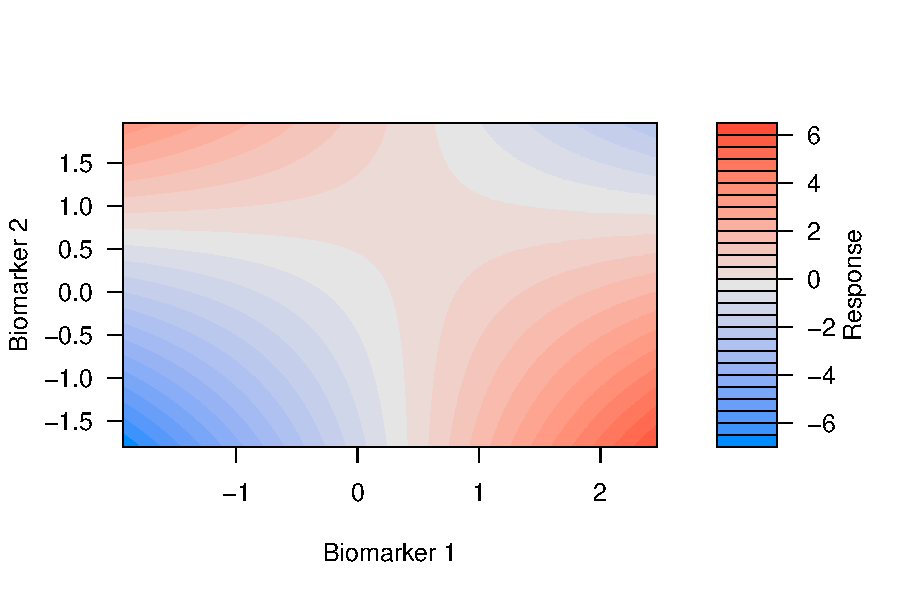
\includegraphics[width=0.75\textwidth]{figura14.pdf}
\caption[Interaction between two variables]{Interaction between two variables (biomarker 1 and biomarker 2). Higher values of one of the two biomarkers are associated to higher values of the response, but only if the other biomarker has not high values either.}
\label{figura14}
\end{figure}

Finally, there is also a concern with the question being asked by the bivariate tests. Usually, what these analysis are doing is flipping the question. If we are looking for biomarkers for detecting a specific disease, we want to be able to predict disease with the value of the biomarkers, this is something inherently different as the question answered by the bivariate hypothesis test: Are the means (medians) for this biomarker different in each group? (\autoref{equation05}). 

\begin{equation}
\label{equation05}
\begin{split}
    Group\ {\raise.17ex\hbox{$\scriptstyle\sim$}}\ Biomarker_i \\
    vs. \phantom{MMMM}  \\
    Biomarker_i\ {\raise.17ex\hbox{$\scriptstyle\sim$}}\ Group
\end{split}
\end{equation}

In the first case, the response variable is the group and the predictors are the different biomarkers. In the second case, the responses are the different biomarkers and the predictor is the group. Since the approaches are different, it is not surprising that the fact that the means are different is not enough to achieve a good discrimination power between groups and, on the other hand, the fact that the means are equal does not mean that the biomarker is not appropriate for discriminating between groups. \autoref{figura15} shows clear examples of both cases.

\begin{figure}[hbtp]
	\centering
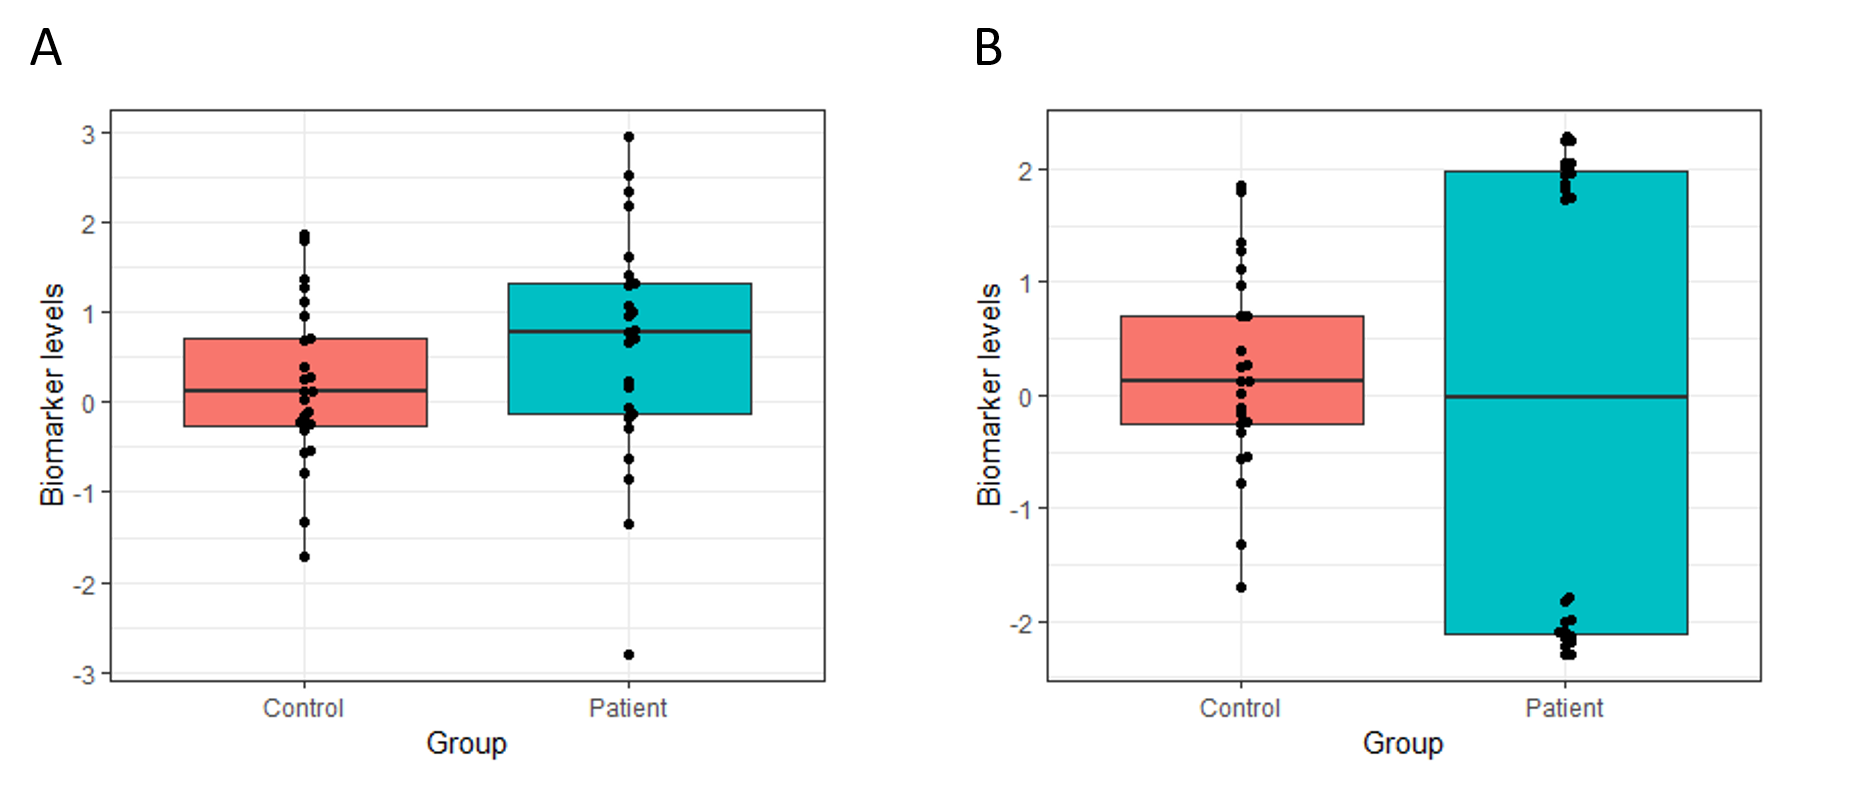
\includegraphics[width=0.95\textwidth]{figura15.png}
\caption[Difference between having different means and discrimination power]{In \textbf{A} means are different (p < 0.001) but values of the biomarker are not valid for discriminationg between controls and patients. In \textbf{B} means are exactly equal, but values of the biomarker allow for a perfect discrimination between both groups.}
\label{figura15}
\end{figure}

In summary, while compelling for their simplicity and ease of use, classical bivariate tests are not appropriate for the analysis of omic data and should only be used in the context of exploratory analysis or complementary secondary analyses.

\section{Linear modelling of omic data}
\label{linearmodels}
Linear models are a generalization of the well known statistical tests \textit{t test} and \textit{ANOVA}, where more predictors can be included in the studied association with the response variable. In fact, the standard \textit{t test} and \textit{ANOVA} are just a linear regression with one categorical predictor (\autoref{figura16})

\begin{figure}[hbtp]
	\centering
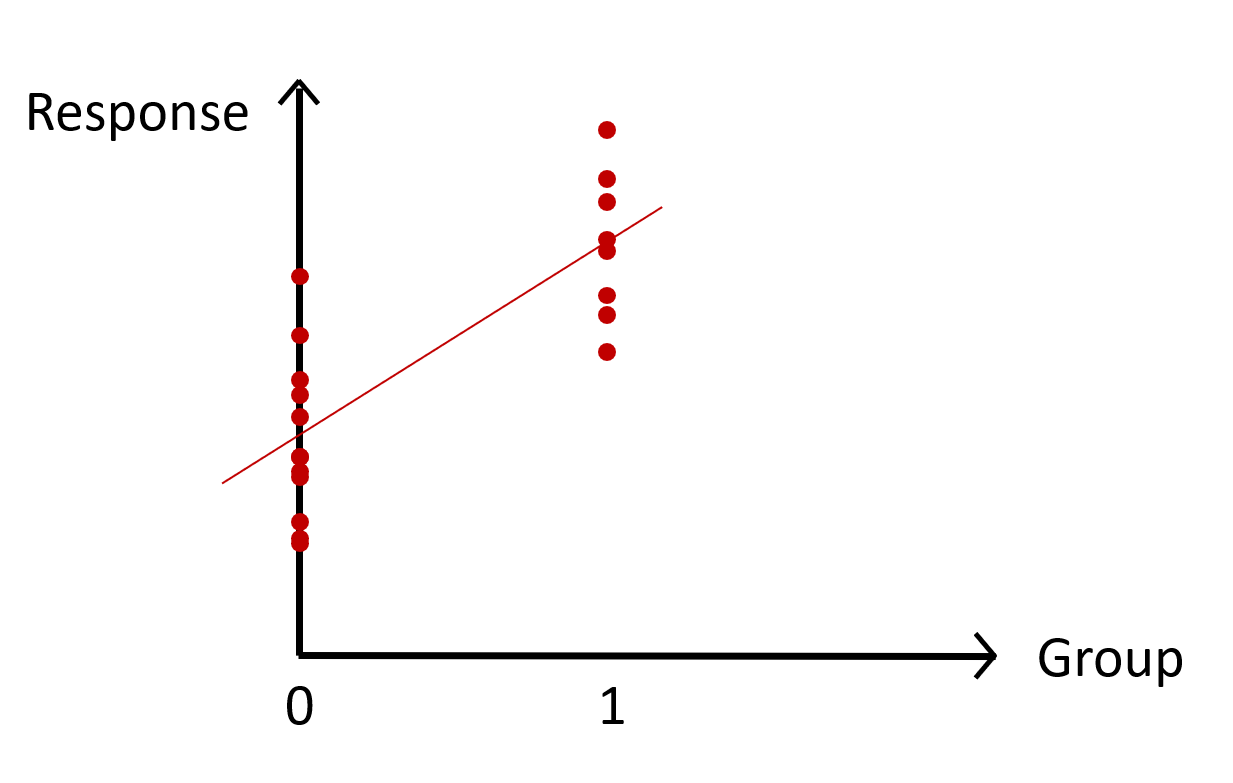
\includegraphics[width=0.75\textwidth]{figura16.png}
\caption[Equivalence between the \textit{t test} and a linear regression with one categorical predictor]{Equivalence between the \textit{t test} and a linear regression with one categorical predictor. It is easy to notice that the slope of the regression line, defined as $\Delta y/\Delta x$, equals the difference between means from group 0 and group 1.}
\label{figura16}
\end{figure}

One advantage of linear models compared to their simpler versions \textit{t test} and \textit{ANOVA} is their ability to control for confounding variables. This overcomes one of the important issues raised in \autoref{bivariate_tests} regarding non-comparable groups in observational studies. The linear model has the form showed in \autoref{equation06}. Where $\beta_0$ is the intercept and $\beta_i$ are the slopes of the different variables included in the model. The linear model can also accommodate interactions by introducing a multiplicative term between variables.

\begin{equation}
\label{equation06}
y=\beta_0 + \beta_i * x_i + \epsilon
\end{equation}

At first glance, it seems like the linear model could solve most of the problems presented in \autoref{bivariate_tests}, including integration of results, capturing interactions and answering the right question. One of the assumptions of linear models is that the response variable is continuous and has a linear relationship with the predictors, but this assumption can be relaxed using a well known generalization of the linear models known as generalized linear models \parencite{mcculloch2000generalized}. This way, it would seem possible to perform regressions to predict or explain relationships of the different metabolites with a continuous variable, and also for discriminating between different groups just by including all studied metabolites in the model as covariates. Unfortunately, linear models cannot accommodate an unlimited number of variables, because they are limited by their degrees of freedom and suffer greatly from overfitting \parencite{babyak2004you, hawkins2004problem}. Thus, in the context of omic data analysis, linear models are only useful for the control of confounding variables. This means that they are used in a similar fashion as the bivariate tests (\autoref{linearmodel}). That is, performing as many regressions as predictor variables are in the data set.

\begin{equation}
\label{linearmodel}
Biomarker_i\ {\raise.17ex\hbox{$\scriptstyle\sim$}}\ Group + Confounder + \epsilon
\end{equation}


\section{Corrections for multiple comparisons}
Each time a hypothesis test is performed, there is a $\alpha\%$ probability of a false positive (usually $\alpha = 0.05$). That means that, when using the techniques presented in \autoref{bivariate_tests} and \autoref{linearmodels}, the probability of false positives grows to unacceptable levels. The relationship between the number of performed hypothesis tests and the overall probability of a false positive is presented in \autoref{falsos_positivos}.

\begin{equation}
\label{falsos_positivos}
    Pr(False\ positive) = 1-(1-\alpha)^{n_{tests}}
\end{equation}

This entails that, in a data set with just 100 variables, we expect five false positives in average. Noteworthy, metabolomic data sets can have up to thousands of variables producing docens or even hundreds of false positives \parencite{broadhurst2006statistical}. This renders the results of the performed hypothesis tests useless, because there is no way of discriminating between false positives and true positives

\subsection{Bonferroni correction}
One method for dealing with the problem of the large number of false positives is the bonferroni correction \parencite{bland1995multiple}. In this method, the $\alpha$ value for each comparison is set to $\alpha /n_{tests}$ in order to control the family wise error rate (the probability of making one or more false discoveries, when performing all the hypothesis tests). So this method is just setting a lower threshold for the significance level. The more hypotheses are tested, the lower is the significance level threshold. This is a very basic correction, and has a major drawback: it greatly increases the number of false negatives. It is straightforward to see that only with 20 tests, the significance level is lowered to $0.05/20 = 0.0025$, so only medium to large effects will be detected assuming that sample size is large enough. But, in the case of metabolomic studies, data sets tend to have many more variables. With 500 variables, the significance level would be $0.05/500=0.0001$ and with 2000 (typical for an untargeted analysis) it would be $0.05/2000=0.000025$. Taking into account the limited sample sizes present in metabolomic studies, only the hugest effects will be detected at such a low significance level \parencite{johnson2010accounting}. 

\subsection{False Discovery Rate}
As explained in the previous paragraph, bonferroni correction greatly increases the number of false negatives. The explanation for this increase can be deduced from the pseudo formula presented in \autoref{error_rates}. In this pseudo formula, both error types are at the same place of the equation and the other parameters are fixed for a specific data set. This means that, when we decrease one of the two error types, the other has to increase accordingly.

\begin{equation}
\label{error_rates}
    N\ {\raise.17ex\hbox{$\scriptstyle\sim$}}\ \frac{variance}{effect\ size + Type\ I\ error + Type\ II\ error}
\end{equation}

In the case of bonferroni correction, the lowering of type I error is huge, so the increase in type II error is correspondingly large. In practice, this usually means that the analysis yields no positive results after a bonferroni correction. To overcome this problem, an alternative, less aggressive correction named False Discovery Rate was developed  \parencite{benjamini1995controlling}. The false discovery rate method is not concerned with the family wise error rate (FWER) as the bonferroni method. It is focused in controlling the number of false positives among all the discovered positives. So, in the case of false discovery rate, we assume that some false positives are going to happen, but want to control their proportion in relation with all the positives. The difference between this approach and the classical control of type I error is explained in \autoref{tableFDR}.

\vspace{10pt}
\begin{table}[h!]
\centering
\begin{tabular}{@{}lcc@{}}
\toprule
                         & \textbf{$H_0$ is true} & \textbf{$H_0$ is false} \\ \midrule
\textbf{Rejected $H_0$}     & FP      & TP        \\
\textbf{Not rejected $H_0$} & TN       & FN       \\ \bottomrule
\end{tabular}
\caption[Difference between FWER and FDR]{Difference between FWER and FDR. FP, TP, TN and FN stand for false positives, true positives, true negatives and false negatives, respectively. In the classic FWER procedures such as bonferroni, one is interested in maintaining the overall proportion of false positives under a specific threshold $\alpha$. In FDR, on the other hand, the interest is in maintaining the ration of FP/(FP+TP) under a specific threshold.}
\label{tableFDR}
\end{table}
\vspace{10pt}

It is easily shown that controlling the ratio FP/(FP+TP) is less stringent than controlling the overall proportion of false positives. Thus, FDR has greater statistical power, although it has a larger amount of type I error compared to bonferroni. This is expected since FDR is also subject to the formula presented in \autoref{error_rates}.

\subsection{Other corrections}
As explained in the preceding paragraph, there is no way out of the formula presented in \autoref{error_rates} when performing hypothesis tests. Several alternative methods have been provided during the last decades \parencite{benjamini2001control, gao2008multiple, castro2015adjusted}, but all of them are just playing with the balance between type I and type II error rate. Some researchers even support that the loss of power is so high, even when performing false discovery rate, that in many cases it would be better to not correct at all and consider the results as exploratory or hypotheses generators instead of forcing an unacceptable low power for confirming hypotheses \parencite{bender2001adjusting}.
In summary, hypothesis testing for the analysis of metabolomic data suffers from many issues that are difficult or, in some cases, impossible to overcome. From the exposed methods in this section, the linear modelling approach seems the most promising, specially when considering its ability to use the different metabolites as predictors, although it would have to overcome its limitation regarding overfitting and limited number of variables due to the degrees of freedom. 

\section{Principal Component analysis}
\label{sec:PCA}
It has already been exposed that linear models could be an appropriate solution for analyzing metabolomic data sets. One of the important issues with them is the saturation of their degrees of freedom when the number of variables is large. Principal component analysis (PCA) is a dimensionality reduction technique, that can be used to reduce the number of variables prior to modeling, thus helping to overcome one of the problems of linear models in the context of high dimensionality data sets \parencite{hotelling1933analysis, wang2008principal}. An illustration of the dimensionality reduction capability of PCA is provided in \autoref{figura33}.


\begin{figure}[hbtp]
	\centering
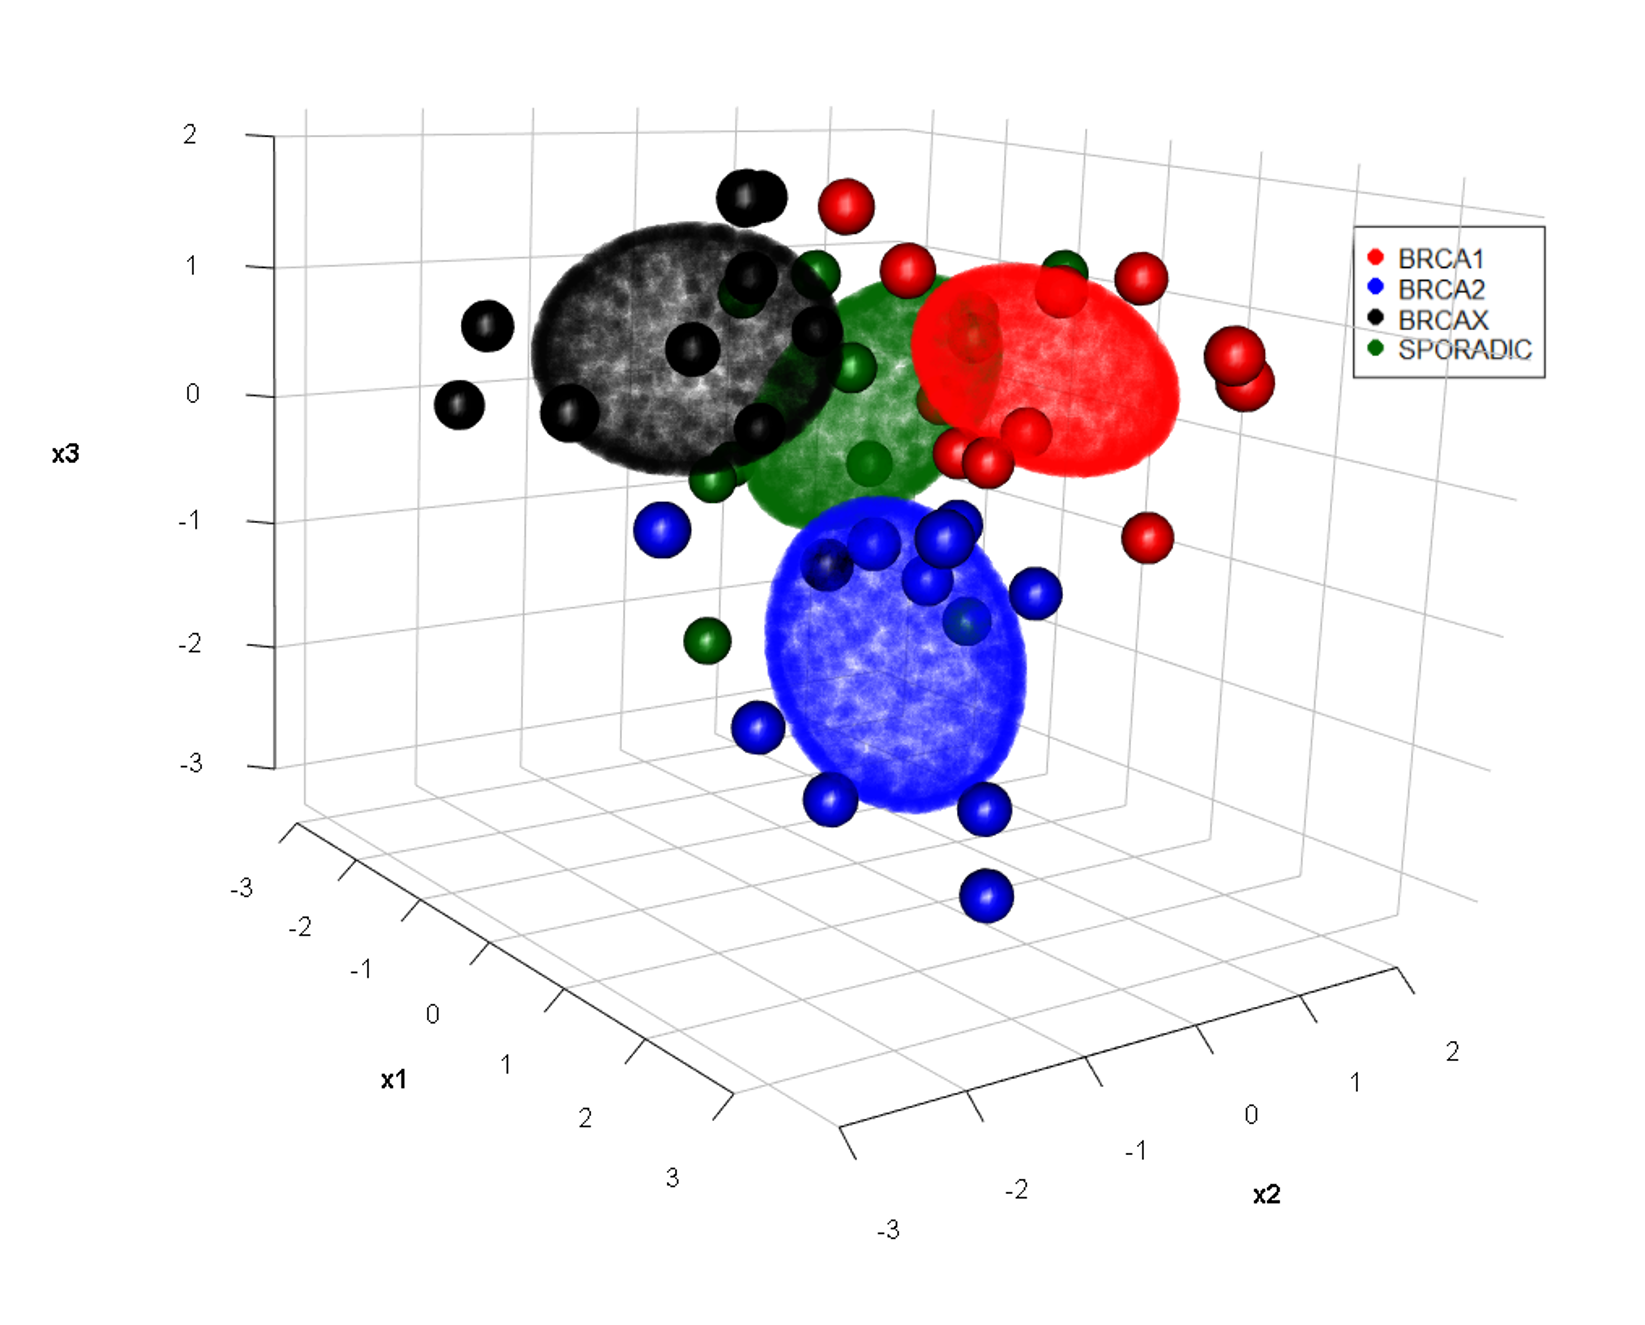
\includegraphics[width=0.75\textwidth]{figura33.png}
\caption[Plot of the first three principal components of a miRNA dataset]{Plot of the first three principal components of a miRNA dataset. These components carry enough information to be able to discriminate four different groups of samples.}
\label{figura33}
\end{figure}

Formally, PCA is defined as an orthogonal linear transformation that projects the data in a new coordinate system such that the greatest variance of the data lies in the first dimension, the second greatest variance in the second dimension, and so on until the number of components is equal to the number of original dimensions. The full principal components decomposition of \textbf{X} is given by (\autoref{equation07}).

\begin{equation}
\label{equation07}
\textbf{\text{T}} = \textbf{\text{XW}}
\end{equation}

Where \textbf{W} is a $p \times p$ matrix of weights whose columns are the eigenvectors of $\textbf{\text{X}}^T\textbf{\text{X}}$. Since the last components are the ones accounting for the least part of the variability, they carry almost no information from the original data matrix. Thus, it is reasonable to remove them keeping only the first components and effectively reducing the dimensionality of the data. Principal component regression then uses these first components as predictors in a linear regression model to predict the response \parencite{jolliffe1982note}.

Another common use of PCA is as an exploratory analysis method \parencite{tsai2007dimensionality}. Since it is very hard to represent more than three dimensions in a surface such as a sheet of paper or a screen, multidimensional data sets such as those coming from omic technologies are difficult to visualize. The dimensionality reduction produced by PCA allows for the representation of such data sets and the performing of exploratory analyses such as outlier detection, batch effect assessment, etc. \parencite{meglen1992examining}.
